\begin{frame}{Transfer learning: Motivation}
    \centering
    Will transfer learning from the pretrained multi-task model result in better predictive performance in downstream prediction tasks relying on small datasets for training?
\end{frame}

\begin{frame}{Transfer learning: Prediction tasks}
    Four prediction tasks:
    \begin{enumerate}
        \item Heterogeneous brain age prediction
        \begin{itemize}
            \item 6,750 images from 20 sources
        \end{itemize}
        \item Homogeneous brain age prediction
        \begin{itemize}
            \item 1,072 images from TOP
        \end{itemize}
        \item Classification of patients with Alzheimer's disease and healthy controls
        \begin{itemize}
            \item 10,660 images from ADNI
        \end{itemize}
        \item Classification of patients with schizophrenia and bipolar disorder
        \begin{itemize}
            \item 1,037 images from TOP
        \end{itemize}
    \end{enumerate}
\end{frame}

\newcommand{\strategynode}[4]{
    \node[
        anchor=west,
        font=\scriptsize\linespread{0.85}\selectfont,
        text width=2cm,
        align=center,
        alt=<#4>{text=black}{text=black!20}
    ] (#1) at #2 {#3};
}

\begin{frame}{Transfer learning: Modelling approaches}
    \begin{tikzpicture}
        \node[] at (-7, -3.25) {};
        \node[] at (7, 3.25) {};

        \strategynode{linear}{(-7, 2.75)}{Linear model}{1}
        \strategynode{baseline}{(linear.east)}{Baseline}{2}
        \strategynode{transferred}{(baseline.east)}{Direct transfer}{3}
        \strategynode{multi-finetune}{(transferred.east)}{Finetuned multi-task model}{4-5}
        \strategynode{reg-finetune}{(multi-finetune.east)}{Finetuned brain age model}{6-7}
        \strategynode{frozen}{(reg-finetune.east)}{Partially finetuned multi-task model}{8-9}

        \inputside{-5.2}{-2}{1.5cm}
        \node[font=\footnotesize] at (-5.2, -0.7) {New data};
        \node[anchor=west, align=left, font=\footnotesize\linespread{0.9}\selectfont] (output) at (3.55, -2) {New task};

        \only<1>{
            \node[fill=gray!20, rounded corners=0.1cm, align=center, font=\footnotesize] (fastsurfer) at (-1.75, -2) {FastSurfer\\segmentation};
            \node[fill=gray!20, rounded corners=0.1cm, align=center, font=\footnotesize] (model) at (1.75, -2) {Linear\\model};
            \node[font=\tiny, align=center, anchor=south] at ($ (fastsurfer.east)!0.5!(model.west) $) {Regional\\volumes};
            \cnnarrow{(input.east)}{(fastsurfer.west)}{black}
            \cnnarrow{(fastsurfer.east)}{(model.west)}{black}
            \cnnarrow{(model.east)}{(output.west)}{black}
        }

        \only<2>{
            \cnnarrow{(input.east)}{($ (input.east) + (3, 0) $)}{black}
            \cnn{-2.7}{-2}{0.1}{0.15}{gray}{0}
            \cnnarrow{($ (output.west) - (1, 0) $)}{(output.west)}{black}
        }
        \only<3-4,6,8>{
            \cnn{-2.7}{0.9}{0.1}{0.15}{uiogreen}{0}
        }
        \only<3-4,8>{
            \node[anchor=west, align=left, font=\footnotesize\linespread{0.9}\selectfont] (output1) at (3.55, 1.9) {Brain age};
            \node[anchor=west, align=left, font=\footnotesize\linespread{0.9}\selectfont] (output2) at (3.55, 1.5) {Sex};
            \node[anchor=west, align=left, font=\footnotesize\linespread{0.9}\selectfont] (output3) at (3.55, 1.1) {Handedness};
            \node[anchor=west, align=left, font=\footnotesize\linespread{0.9}\selectfont] (output4) at (3.55, 0.7) {BMI};
            \node[anchor=west, align=left, font=\footnotesize\linespread{0.9}\selectfont] (output5) at (3.55, 0.3) {Fluid intelligence};
            \node[anchor=west, align=left, font=\footnotesize\linespread{0.9}\selectfont] (output6) at (3.55, -0.1) {Neuroticism};

            \cnnarrow{($ (output1.west) - (1, 1) $)}{(output1.west)}{black}
            \cnnarrow{($ (output2.west) - (1, 0.6) $)}{(output2.west)}{black}
            \cnnarrow{($ (output3.west) - (1, 0.2) $)}{(output3.west)}{black}
            \cnnarrow{($ (output4.west) - (1, -0.2) $)}{(output4.west)}{black}
            \cnnarrow{($ (output5.west) - (1, -0.6) $)}{(output5.west)}{black}
            \cnnarrow{($ (output6.west) - (1, -1) $)}{(output6.west)}{black}
        }
        \only<3-4,6,8>{
            \draw[-stealth, uiolightred, line width=0.5, line width=4pt] (-1.75, -0.2) -- (-1.75, -0.85);
            \draw[-stealth, uiolightred, line width=0.5, line width=4pt] (-0.25, 0.05) -- (-0.25, -1.075);
            \draw[-stealth, uiolightred, line width=0.5, line width=4pt] (0.85, 0.4) -- (0.85, -1.525);
            \draw[-stealth, uiolightred, line width=0.5, line width=4pt] (2.1, 0.6) -- (2.1, -1.75);
        }
        \only<3-4,6,8>{
            \cnnarrow{(input.east)}{($ (input.east) + (3, 0) $)}{black}
            \cnn{-2.7}{-2}{0.1}{0.15}{uiogreen}{0}
            \cnnarrow{($ (output.west) - (1, 0) $)}{(output.west)}{black}
        }
        \only<5,7>{
            \cnnarrow{(input.east)}{($ (input.east) + (3, 0) $)}{black}
            \cnn{-2.7}{-2}{0.1}{0.15}{uiored}{0}
            \cnnarrow{($ (output.west) - (1, 0) $)}{(output.west)}{black}
        }
        \only<6>{
            \node[anchor=west, align=left, font=\footnotesize\linespread{0.9}\selectfont] (output1) at (3.55, 0.9) {Brain age};
            \cnnarrow{($ (output1.west) - (1, 0) $)}{(output1.west)}{black}
        }
        \only<9>{
            \cnnarrow{(input.east)}{($ (input.east) + (3, 0) $)}{black}
            \cnn{-2.7}{-2}{0.1}{0.15}{uiogreen}{0}
            \cnnarrow{($ (output.west) - (1, 0) $)}{(output.west)}{red}
        }

    \end{tikzpicture}
\end{frame}

\begin{frame}{Transfer learning: Sampling}
    \begin{tikzpicture}
        \node[] at (-7, -3.25) {};
        \node[] at (7, 3.25) {};

        \only<1-5>{
            \stickman{(-4.5, -1.7)}{gray}
            \stickman{(-3.8, -1.8)}{gray}
            \stickman{(-2.5, -1.6)}{gray}
            \stickman{(-1.8, -1.9)}{gray}
            \stickman{(0.7, -1.8)}{gray}
            \stickman{(3.1, -1.5)}{gray}
            \stickman{(3.6, -2)}{gray}
            \stickman{(4.5, -1.9)}{gray}

            \stickman{(-3.8, -0.6)}{gray}
            \stickman{(-2.6, -0.4)}{gray}
            \stickman{(-2.1, -0.5)}{gray}
            \stickman{(0.1, -0.3)}{gray}
            \stickman{(1, -0.8)}{gray}
            \stickman{(2.6, -0.4)}{gray}
            \stickman{(4.4, -0.3)}{gray}

            \stickman{(-4.2, 0.4)}{gray}
            \stickman{(0.5, 0.6)}{gray}
            \stickman{(1.9, 0.7)}{gray}
        }
        \only<2->{
            \node[] at (0, 3) {\underline{n=$100$}};
        }
        \only<1-3>{
            \stickman{(-3, -1.2)}{gray}
            \stickman{(0, -1.6)}{gray}
            \stickman{(2.2, -1.3)}{gray}
            \stickman{(-4.6, -0.5)}{gray}
            \stickman{(-1, -0.9)}{gray}
            \stickman{(1.5, -0.2)}{gray}
            \stickman{(3.1, -0.1)}{gray}
            \stickman{(3.6, -0.8)}{gray}
            \stickman{(-2.5, 0.8)}{gray}
            \stickman{(3.8, 0.5)}{gray}
        }
        \only<1-4>{
            \stickman{(-0.5, -0.1)}{gray}
            \stickman{(-1.5, 0.1)}{gray}
        }
        \only<1-5>{
            \stickman{(-3.2, 0.6)}{gray}
            \stickman{(1.3, -1.9)}{gray}
        }
        \only<3->{
            \stickman{(-4.225, 2.25)}{uioblue}
            \stickman{(-3.575, 2.25)}{uioblue}
            \stickman{(-2.925, 2.25)}{uioblue}
            \stickman{(-2.275, 2.25)}{uioblue}
            \stickman{(-1.625, 2.25)}{uioblue}
            \stickman{(-0.975, 2.25)}{uioblue}
            \stickman{(-0.325, 2.25)}{uioblue}
            \stickman{(0.325, 2.25)}{uioblue}
            \stickman{(0.975, 2.25)}{uioblue}
            \stickman{(1.625, 2.25)}{uioblue}
        }
        \only<3-5>{
            \stickman{(-3, -1.2)}{uioblue}
            \stickman{(0, -1.6)}{uioblue}
            \stickman{(2.2, -1.3)}{uioblue}
            \stickman{(-4.6, -0.5)}{uioblue}
            \stickman{(-1, -0.9)}{uioblue}
            \stickman{(1.5, -0.2)}{uioblue}
            \stickman{(3.1, -0.1)}{uioblue}
            \stickman{(3.6, -0.8)}{uioblue}
            \stickman{(-2.5, 0.8)}{uioblue}
            \stickman{(3.8, 0.5)}{uioblue}
        }
        \only<4->{
            \stickman{(2.275, 2.25)}{uioorange}
            \stickman{(2.925, 2.25)}{uioorange}
        }
        \only<4-5>{
            \stickman{(-0.5, -0.1)}{uioorange}
            \stickman{(-1.5, 0.1)}{uioorange}
        }
        \only<5->{
            \stickman{(3.575, 2.25)}{uiored}
            \stickman{(4.225, 2.25)}{uiored}
        }
        \only<5>{
            \stickman{(-3.2, 0.6)}{uiored}
            \stickman{(1.3, -1.9)}{uiored}
        }
        \only<6->{
            \node[font=\footnotesize] (error1) at (6, 1.9) {Error};
        }
        \only<6>{
            \node[fill=gray!20, rounded corners=0.1cm, font=\footnotesize] (train) at (-1.3, -0.5) {
                Train
            };
            \node[fill=gray!20, rounded corners=0.1cm, font=\footnotesize] (validate) at (2.6, -0.5) {
                Validate
            };
            \node[fill=gray!20, rounded corners=0.1cm, font=\footnotesize] (test) at (3.9, -0.5) {
                Test
            };
            \draw[-stealth, dashed] ($ (train.north) + (0, 1.5) $) -- (train.north);
            \draw[-stealth, dashed] ($ (validate.north) + (0, 1.5) $) -- (validate.north);
            \draw[-stealth, dashed] ($ (test.north) + (0, 1.5) $) -- (test.north);
            \draw[-stealth] (train) -- (validate);
            \draw[-stealth] (validate) -- (test);
            \draw[-stealth] (test.east) -| (error1);
        }
        \only<7->{
            \stickman{(-4.225, 1)}{uioblue}
            \stickman{(-3.575, 1)}{uioblue}
            \stickman{(-2.925, 1)}{uioblue}
            \stickman{(-2.275, 1)}{uioblue}
            \stickman{(-1.625, 1)}{uioblue}
            \stickman{(-0.975, 1)}{uioblue}
            \stickman{(-0.325, 1)}{uioblue}
            \stickman{(0.325, 1)}{uioblue}
            \stickman{(0.975, 1)}{uioblue}
            \stickman{(1.625, 1)}{uioblue}
            \stickman{(2.275, 1)}{uioorange}
            \stickman{(2.925, 1)}{uioorange}
            \stickman{(3.575, 1)}{uiored}
            \stickman{(4.225, 1)}{uiored}
        }
        \only<8->{
            \node[font=\footnotesize] (error2) at (6, 0.65) {Error};
        }
        \only<8>{
            \node[fill=gray!20, rounded corners=0.1cm, font=\footnotesize] (train) at (-1.3, -1.75) {
                Train
            };
            \node[fill=gray!20, rounded corners=0.1cm, font=\footnotesize] (validate) at (2.6, -1.75) {
                Validate
            };
            \node[fill=gray!20, rounded corners=0.1cm, font=\footnotesize] (test) at (3.9, -1.75) {
                Test
            };
            \draw[-stealth, dashed] ($ (train.north) + (0, 1.5) $) -- (train.north);
            \draw[-stealth, dashed] ($ (validate.north) + (0, 1.5) $) -- (validate.north);
            \draw[-stealth, dashed] ($ (test.north) + (0, 1.5) $) -- (test.north);
            \draw[-stealth] (train) -- (validate);
            \draw[-stealth] (validate) -- (test);
            \draw[-stealth] (test.east) -| (error2);
        }
        \only<9->{
            \stickman{(-4.225, -0.25)}{uioblue}
            \stickman{(-3.575, -0.25)}{uioblue}
            \stickman{(-2.925, -0.25)}{uioblue}
            \stickman{(-2.275, -0.25)}{uioblue}
            \stickman{(-1.625, -0.25)}{uioblue}
            \stickman{(-0.975, -0.25)}{uioblue}
            \stickman{(-0.325, -0.25)}{uioblue}
            \stickman{(0.325, -0.25)}{uioblue}
            \stickman{(0.975, -0.25)}{uioblue}
            \stickman{(1.625, -0.25)}{uioblue}
            \stickman{(2.275, -0.25)}{uioorange}
            \stickman{(2.925, -0.25)}{uioorange}
            \stickman{(3.575, -0.25)}{uiored}
            \stickman{(4.225, -0.25)}{uiored}

            \node[font=\footnotesize] (error3) at (6, -0.6) {Error};

            \node[font=\small] at (0, -1.5) {x50};

            \draw[red, dashed] (error1.north west) -- (error1.north east) -- (error3.south east) -- (error3.south west) -- cycle;
        }
        \only<10>{
            \node[] at (0, -2.25) {\underline{n=$200$}};
            \node[] at (0, -3) {\underline{n=$300$}};
        }

    \end{tikzpicture}
\end{frame}

\newcommand{\resultstrace}[3]{
    \addplot+[
        scatter,
        draw=#2,
        mark=#3,
        thick,
        draw opacity=0.75,
        visualization depends on={\thisrow{#2-significant} \as \significant},
        scatter/@pre marker code/.code={
            \pgfplotscolormapdefinemappedcolor\pgfplotspointmetatransformed
            \def\markopts{
                fill=#2,
                fill opacity=0.75*\significant,
                mark size=4pt
            }
            \expandafter\scope\expandafter[\markopts]
        },
    ] table [
        col sep=comma,
        x=size,
        y=#2-median,
        meta=#2-significant
    ] {#1};
}
\newcommand{\legendtrace}[3][0.75]{
    \begin{tikzpicture}[baseline={([yshift=-0.125cm]current bounding box.center)}]
        \draw[draw=#2, thick] (0cm, 0cm) -- (0.5cm, 0cm);

        \path[
            mark=#3,
            mark size=4pt,
            mark options={fill=#2, draw=#2},
            fill opacity=#1
        ] plot coordinates {(0.25cm, 0cm)};
    \end{tikzpicture}
}

\newcommand{\legendnode}[4][north east]{
    \node[draw=black, fill=white, anchor=#1, font=\fontsize{6}{5}\selectfont, text width=3.3cm] at (#2) {
        \vspace{-0.07cm}
        \setlength\tabcolsep{0cm}
        \renewcommand{\arraystretch}{1.8}
        \begin{tabular}{p{0.53cm} p{2.8cm}}
            #3
        \end{tabular}
        \vspace{0.2cm}\\
        \begin{tabular}{p{0.53cm} p{2.8cm}}
            #4
        \end{tabular}
    };
}

\definecolor{multi-transferred}{RGB}{213, 94, 0}
\definecolor{multi-frozen}{RGB}{0, 158, 115}
\definecolor{multi-finetuned}{RGB}{86, 180, 233}
\definecolor{reg-finetuned}{RGB}{213, 94, 0}
\definecolor{baseline}{RGB}{230, 159, 0}
\definecolor{linear}{RGB}{64, 64, 64}

\makeatletter
\pgfdeclareplotmark{triangledown*}{
  \pgfpathmoveto{\pgfpoint{0}{-1.2\pgfplotmarksize}}
  \pgfpathlineto{\pgfpoint{1.04\pgfplotmarksize}{0.6\pgfplotmarksize}}
  \pgfpathlineto{\pgfpoint{-1.04\pgfplotmarksize}{0.6\pgfplotmarksize}}
  \pgfpathclose
  \pgfusepathqfillstroke
}
\makeatother

\def\multifrozenmarker{*}
\def\regfinetunedmarker{square*}
\def\multifinetunedmarker{pentagon*}
\def\multitransferredmarker{triangle*}
\def\linearmarker{triangledown*}
\def\baselinemarker{diamond*}


\begin{frame}{Results: Heterogeneous brain age predictions}
    \centering
    \begin{tikzpicture}
        \begin{axis}[
            height=6.25cm,
            width=12cm,
            ymajorgrids=true,
            xlabel={Training dataset size},
            ylabel={Relative absolute error},
            tick style={draw=none},
            ymin=0.1,
            xtick={100, 250, 500, 1000, 2500},
            xticklabel style={
                rotate=45,
                anchor=north east
            },
            xlabel style={
                yshift=0.1cm
            }
        ]
            \resultstrace{data/downstream/age/results.csv}{baseline}{\baselinemarker}
            \node[draw=black, fill=white, anchor=north east, text width=4cm, inner sep=2pt, font=\footnotesize] at (rel axis cs: 0.98, 0.98) {
                \setlength\tabcolsep{0cm}%
                \begin{tabular}{cl}
                    \legendtrace{baseline}{\baselinemarker} & Baseline\\
                    \visible<2->{\legendtrace{multi-finetuned}{\multifinetunedmarker}} & \visible<2->{Finetuned multi-task}\\
                    \visible<3->{\legendtrace{multi-frozen}{\multifrozenmarker}} & \visible<3->{Frozen multi-task}\\
                    \visible<3->{\legendtrace{multi-transferred}{\multitransferredmarker}} & \visible<3->{Transferred multi-task}\\[0.2cm]
                    \visible<2->{\legendtrace[0]{black}{*}}&\visible<2->{\hspace{0.1cm}$p\geq0.05$}\\
                    \visible<2->{\legendtrace{black}{*}}&\visible<2->{\hspace{0.1cm}$p<0.05$}\\
                \end{tabular}

            };
            \only<2->{
                \resultstrace{data/downstream/age/results.csv}{multi-finetuned}{\multifinetunedmarker}
            }
            \only<3->{
                \resultstrace{data/downstream/age/results.csv}{multi-frozen}{\multifrozenmarker}
                \resultstrace{data/downstream/age/results.csv}{multi-transferred}{\multitransferredmarker}
            }

        \end{axis}
    \end{tikzpicture}
\end{frame}

\begin{frame}{Results: Homogeneous brain age predictions}
    \centering
    \begin{tikzpicture}
        \begin{axis}[
            height=7cm,
            width=12cm,
            ymajorgrids=true,
            xlabel={Training dataset size},
            ylabel={Relative absolute error},
            tick style={draw=none},
            ymin=0.4,
            xtick={100, 200, 300, 400, 500},
            xlabel style={
                yshift=0.1cm
            }
        ]
            \resultstrace{data/downstream/age_top/results.csv}{baseline}{\baselinemarker}
            \node[draw=black, fill=white, anchor=north east, text width=4cm, inner sep=2pt, font=\footnotesize] at (rel axis cs: 0.98, 0.98) {
                \setlength\tabcolsep{0cm}%
                \begin{tabular}{cl}
                    \legendtrace{baseline}{\baselinemarker} & Baseline\\
                    \visible<2->{\legendtrace{multi-transferred}{\multitransferredmarker}} & \visible<2->{Transferred multi-task}\\
                    \visible<3->{\legendtrace{multi-finetuned}{\multifinetunedmarker}} & \visible<3->{Finetuned multi-task}\\
                    \visible<4->{\legendtrace{multi-frozen}{\multifrozenmarker}} & \visible<4->{Frozen multi-task}\\
                \end{tabular}

            };
            \only<2->{
                \resultstrace{data/downstream/age_top/results.csv}{multi-transferred}{\multitransferredmarker}
            }
            \only<3->{
                \resultstrace{data/downstream/age_top/results.csv}{multi-finetuned}{\multifinetunedmarker}
            }
            \only<4->{
                \resultstrace{data/downstream/age_top/results.csv}{multi-frozen}{\multifrozenmarker}
            }

        \end{axis}
    \end{tikzpicture}
\end{frame}

\begin{frame}{Results: Brain age}
    If you want to accurately predict brain age in new samples:
    \begin{itemize}
        \item You should \textit{always} use a pretrained model
        \item In smaller, homogeneous, samples the model should ideally be finetuned, but using a pretrained model off-the-shelf works reasonably well
    \end{itemize}
\end{frame}

\begin{frame}{Results: AD vs HC classification}
    \centering
    \begin{tikzpicture}
        \begin{axis}[
            height=7cm,
            width=12cm,
            ymajorgrids=true,
            xlabel={Training dataset size},
            ylabel={Area under the ROC-curve},
            tick style={draw=none},
            xtick={100, 200, 300, 400, 500},
            xlabel style={
                yshift=0.1cm
            },
            ymin=0.65,
            ymax=0.97
        ]
            \resultstrace{data/downstream/ad/results.csv}{baseline}{\baselinemarker}
            \node[draw=black, fill=white, anchor=south east, text width=4cm, inner sep=2pt, font=\footnotesize] at (rel axis cs: 0.98, 0.02) {
                \setlength\tabcolsep{0cm}%
                \begin{tabular}{cl}
                    \legendtrace{baseline}{\baselinemarker} & Baseline\\
                    \visible<2->{\legendtrace{multi-frozen}{\multifrozenmarker}} & \visible<2->{Frozen multi-task}\\
                    \visible<3->{\legendtrace{reg-finetuned}{\regfinetunedmarker}} & \visible<3->{Finetuned brain age}\\
                    \visible<4->{\legendtrace{multi-finetuned}{\multifinetunedmarker}} & \visible<4->{Finetuned multi-task}\\
                    \visible<5->{\legendtrace{linear}{\linearmarker}} & \visible<5->{Linear}\\
                \end{tabular}

            };
            \only<2->{
                \resultstrace{data/downstream/ad/results.csv}{multi-frozen}{\multifrozenmarker}
            }
            \only<3->{
                \resultstrace{data/downstream/ad/results.csv}{reg-finetuned}{\regfinetunedmarker}
            }
            \only<4->{
                \resultstrace{data/downstream/ad/results.csv}{multi-finetuned}{\multifinetunedmarker}
            }
            \only<5->{
                \resultstrace{data/downstream/ad/results.csv}{linear}{\linearmarker}
            }

        \end{axis}
    \end{tikzpicture}
\end{frame}

\begin{frame}{Results: SCZ vs BD classification}
    \centering
    \begin{tikzpicture}
        \begin{axis}[
            height=7cm,
            width=12cm,
            ymajorgrids=true,
            xlabel={Training dataset size},
            ylabel={Area under the ROC-curve},
            tick style={draw=none},
            xtick={100, 200, 300, 400, 500},
            xlabel style={
                yshift=0.1cm
            },
            ymin=0.45,
            ymax=0.72
        ]
            \resultstrace{data/downstream/scz/results.csv}{baseline}{\baselinemarker}
            \node[draw=black, fill=white, anchor=south east, text width=4cm, inner sep=2pt, font=\footnotesize] at (rel axis cs: 0.98, 0.02) {
                \setlength\tabcolsep{0cm}%
                \begin{tabular}{cl}
                    \legendtrace{baseline}{\baselinemarker} & Baseline\\
                    \visible<2->{\legendtrace{multi-frozen}{\multifrozenmarker}} & \visible<2->{Frozen multi-task}\\
                    \visible<3->{\legendtrace{multi-finetuned}{\multifinetunedmarker}} & \visible<3->{Finetuned multi-task}\\
                    \visible<3->{\legendtrace{linear}{\linearmarker}} & \visible<3->{Linear}\\
                \end{tabular}

            };
            \only<2->{
                \resultstrace{data/downstream/scz/results.csv}{multi-frozen}{\multifrozenmarker}
            }
            \only<3->{
                \resultstrace{data/downstream/scz/results.csv}{multi-finetuned}{\multifinetunedmarker}
            }
            \only<4->{
                \resultstrace{data/downstream/scz/results.csv}{linear}{\linearmarker}
            }

        \end{axis}
    \end{tikzpicture}
\end{frame}

\begin{frame}{Results: Brain age}
    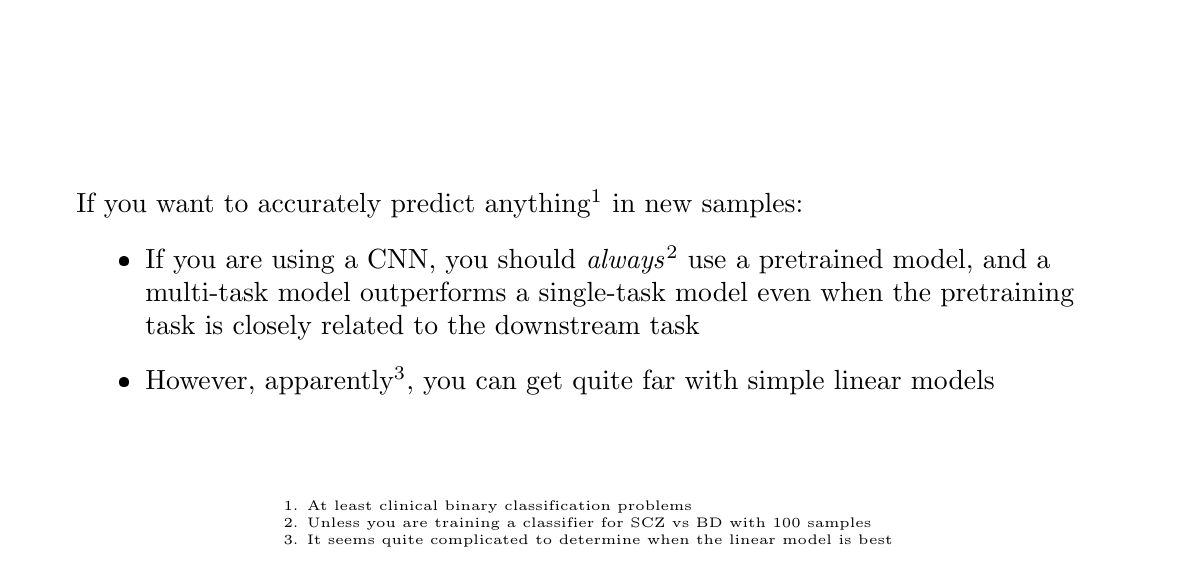
\begin{tikzpicture}
        \node[] at (-7, -3.25) {};
        \node[] at (7, 3.25) {};

        \node[text width=13cm] at (0, 0) {
            If you want to accurately predict anything\textsuperscript{1} in new samples:
            \begin{itemize}
                \item If you are using a CNN, you should \textit{always}\textsuperscript{2} use a pretrained model, and a multi-task model outperforms a single-task model even when the pretraining task is closely related to the downstream task
                \item However, apparently\textsuperscript{3}, you can get quite far with simple linear models
            \end{itemize}
        };
        \node[font=\tiny, anchor=south, align=left] at (0, -3.35) {
            1. At least clinical binary classification problems\\
            2. Unless you are training a classifier for SCZ vs BD with 100 samples\\
            3. It seems quite complicated to determine when the linear model is best
        };
    \end{tikzpicture}
\end{frame}